%%%%%%%%%%%%%%%%%%%%%%%%%%%%%%%%%%%%%%%%%
% Beamer Presentation
% LaTeX Template
% Version 1.0 (10/11/12)
%
% This template has been downloaded from:
% http://www.LaTeXTemplates.com
%
% License:
% CC BY-NC-SA 3.0 (http://creativecommons.org/licenses/by-nc-sa/3.0/)
%
%%%%%%%%%%%%%%%%%%%%%%%%%%%%%%%%%%%%%%%%%

%----------------------------------------------------------------------------------------
%	PACKAGES AND THEMES
%----------------------------------------------------------------------------------------

\documentclass{beamer}

\mode<presentation> {
\usetheme{Madrid}
}

\usepackage{graphicx} % Allows including images
\usepackage{booktabs} % Allows the use of \toprule, \midrule and \bottomrule in tables
\usepackage{multirow}
\usepackage{pdfpages}
\usepackage{tikz}
\usetikzlibrary{shapes.geometric, arrows, positioning, fit}
\newcommand{\bx}{\boldsymbol{x}}
\newcommand{\by}{\boldsymbol{y}}
\newcommand{\bX}{\boldsymbol{X}}
\newcommand{\bY}{\boldsymbol{Y}}

\newcommand{\xmark}{\textcolor{red}{\text{\sffamily X}}}
\newcommand{\cmark}{\textcolor{green}{\checkmark}}
\newcommand{\tr}{\text{tr}}
\newcommand{\E}{\textbf{E}}
\newcommand{\diag}{\text{diag}}
\newcommand{\argmax}{\text{argmax}}
\newcommand{\argmin}{\text{argmin}}
\newcommand{\Cov}{\text{Cov}}
\newcommand{\Vol}{\text{Vol}}

%----------------------------------------------------------------------------------------
%	TITLE PAGE
%----------------------------------------------------------------------------------------


\title[Proposal]{Reverse-engineering the brain}

\author{Charles Zheng} % Your name
\institute[Stanford] % Your institution as it will appear on the bottom of every slide, may be shorthand to save space
{Stanford University}
\date{\today} % Date, can be changed to a custom date

\begin{document}

\begin{frame}
\titlepage % Print the title page as the first slide
\end{frame}

\section{Introduction}
{
\setbeamercolor{background canvas}{bg=}
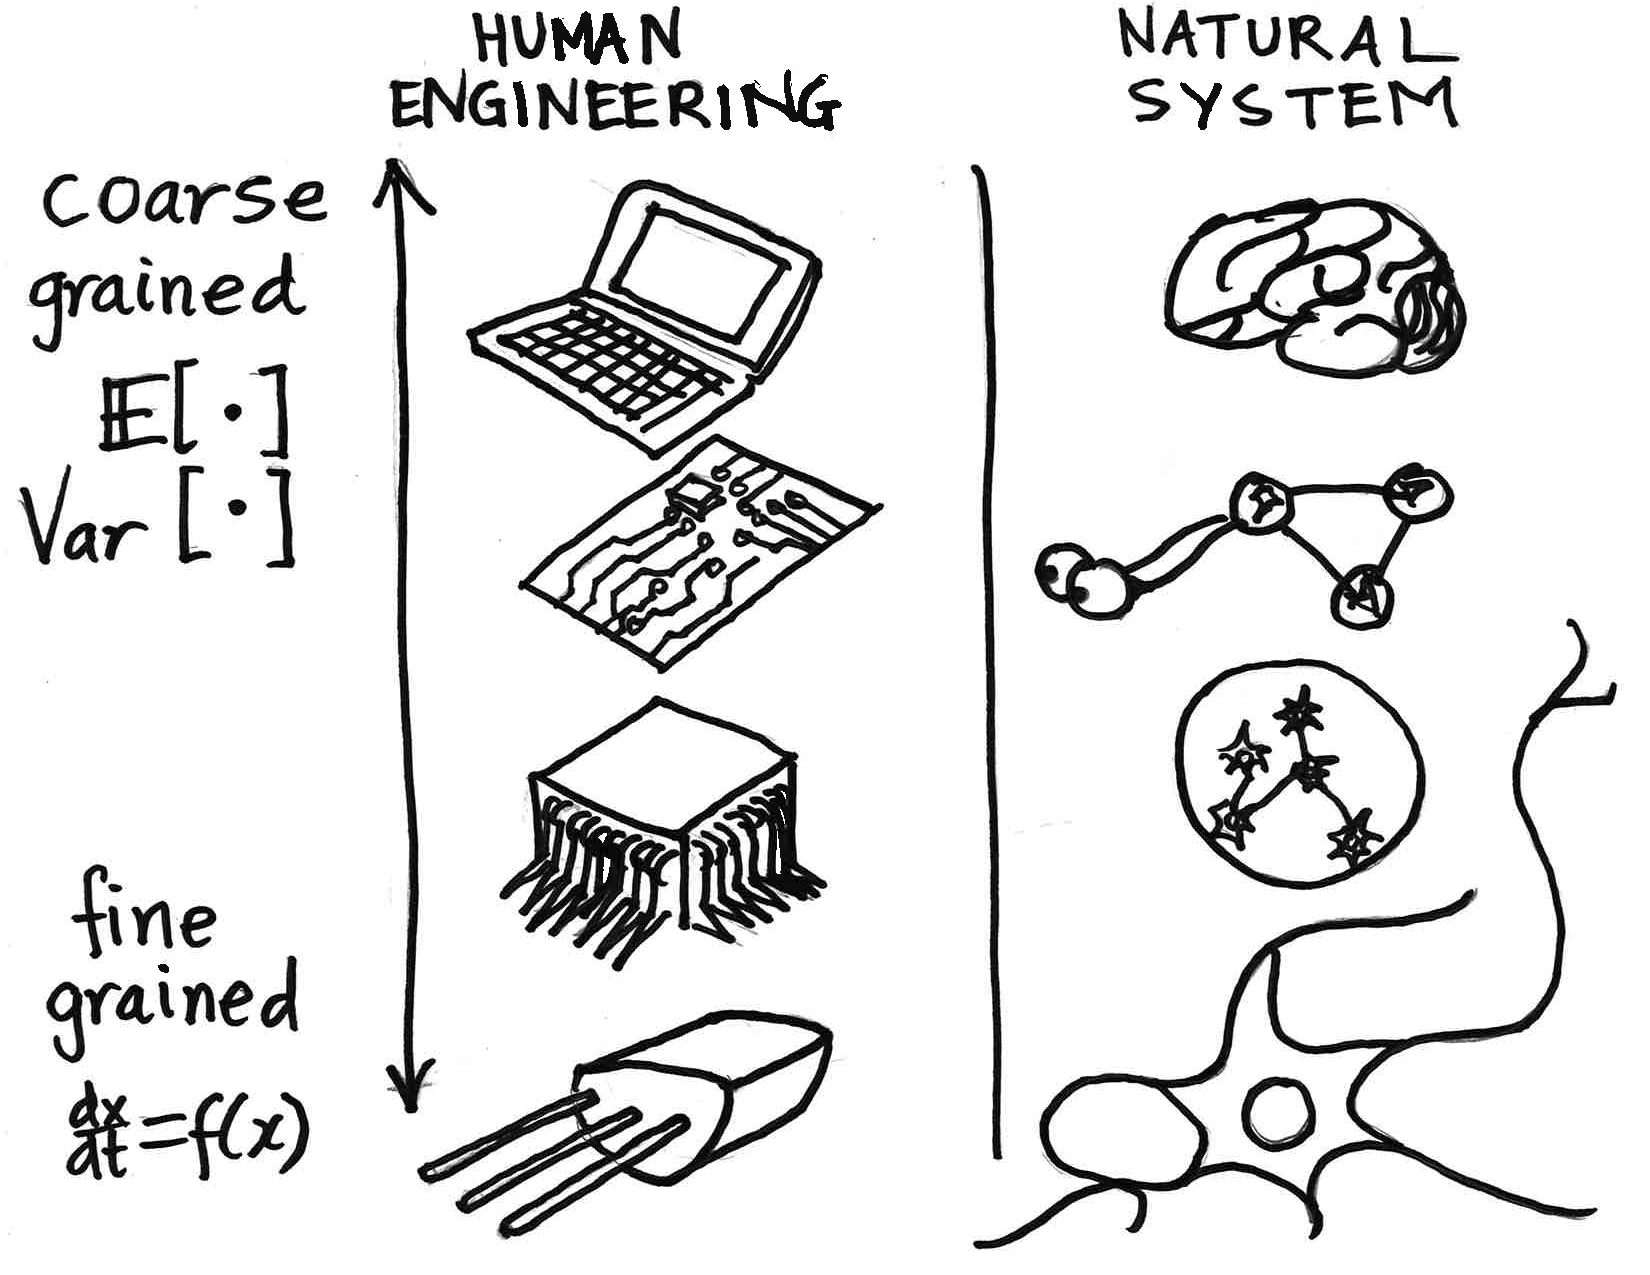
\includepdf[pages=1]{sketch.pdf}
}

\begin{frame}
\frametitle{Levels of Model Building}
\begin{center}
\begin{tabular}{c|c|c}
Level & Neuroscience & Statistics\\
\hline
Reductionist & Segmentation & Clustering\\
Topological & Connectomics & Graphical Lasso\\
Information Flow & RSA? & \textbf{this thesis!}\\
Explicit Mechanisms & Encoding models & Regression
\end{tabular}
\end{center}
\end{frame}

{
\setbeamercolor{background canvas}{bg=}
\includepdf[pages=2-4]{sketch.pdf}
}

\begin{frame}
\frametitle{Functional MRI}
\begin{center}
\begin{tabular}{ccc}
\hline
Stimuli $x$ & & Response $y$\\ \hline
$\begin{pmatrix}1.0 \\ 0 \\ 3.0 \\ 0\\ -1.2\end{pmatrix}$ & \hspace{1in} & $\begin{pmatrix}1.2 \\ 0 \\ -1.8\\ -1.2\end{pmatrix}$ \\ \hline
$\begin{pmatrix}0 \\ -2.2 \\ -3.1 \\ 4.5\\ 0\end{pmatrix}$ & \hspace{1in} & $\begin{pmatrix}-1.2 \\ -1.9\\ 0.5\\ 0.6\end{pmatrix}$ \\ \hline
\hspace{1in} & \hspace{1in} & \hspace{1in}
\end{tabular}
\end{center}
\end{frame}

{
\setbeamercolor{background canvas}{bg=}
\includepdf[pages=5-6]{sketch.pdf}
}

\begin{frame}
\frametitle{A mind-reading game: Classification}
\begin{center}
Training Data
\\
\begin{tabular}{ccc||ccc}
\hline
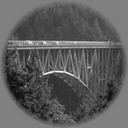
\includegraphics[scale = .26]{img1.png} & \hspace{0.2in} & 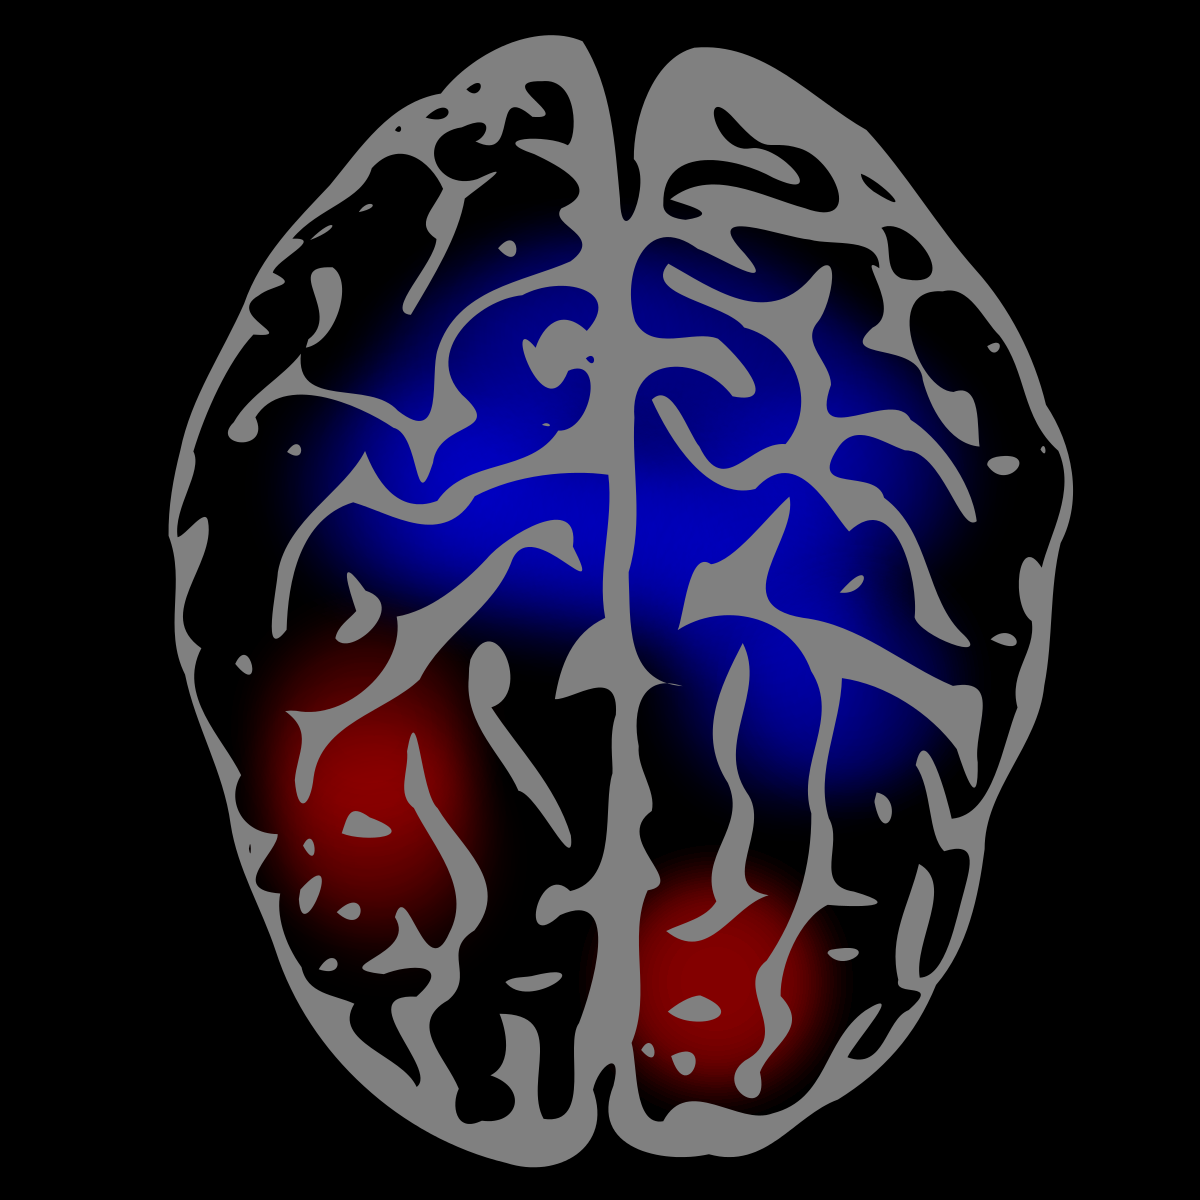
\includegraphics[scale = 0.035]{brain1.png} &
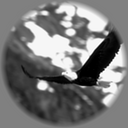
\includegraphics[scale = .26]{img3.png} & \hspace{0.2in} & 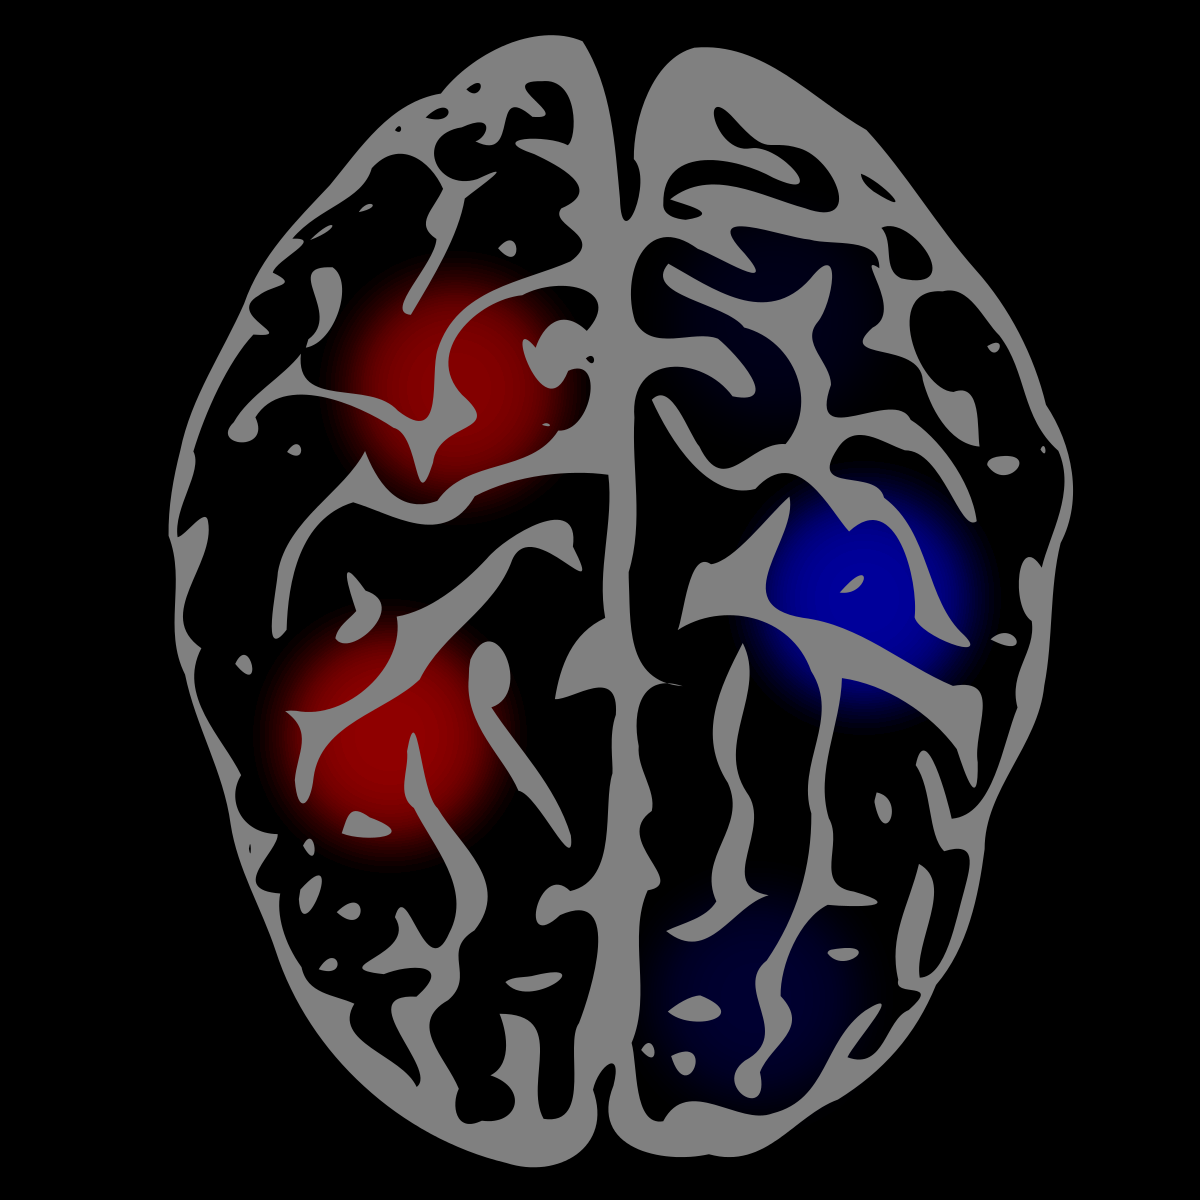
\includegraphics[scale = 0.035]{brain3.png} \\ \hline
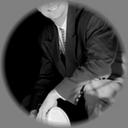
\includegraphics[scale = .26]{img2.png} & \hspace{0.2in} & 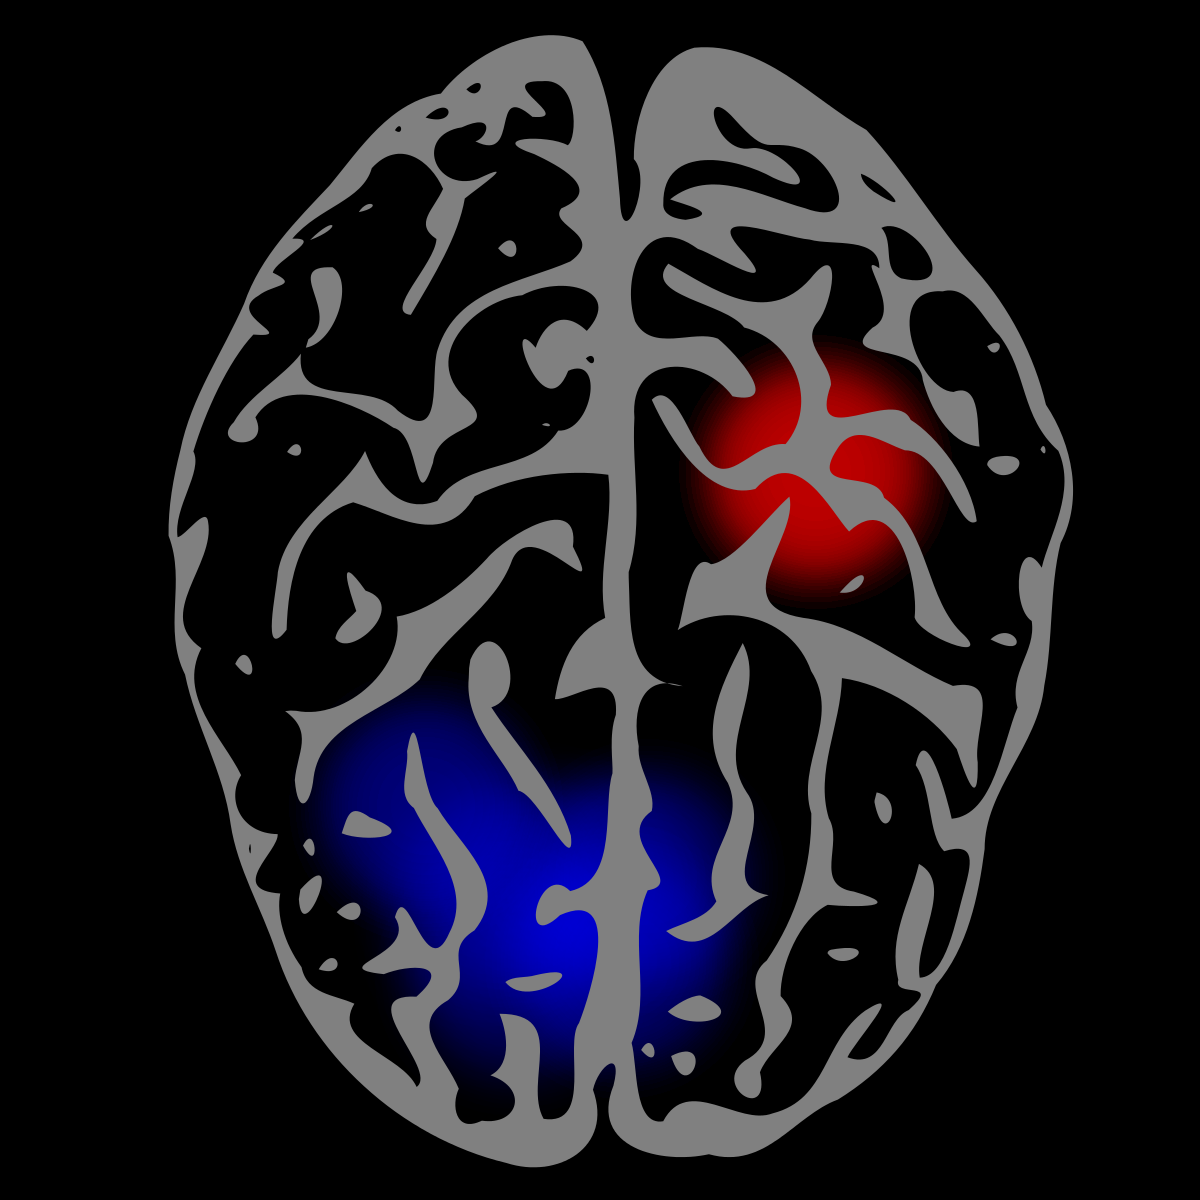
\includegraphics[scale = 0.035]{brain2.png} &
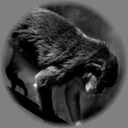
\includegraphics[scale = .26]{img4.png} & \hspace{0.2in} & 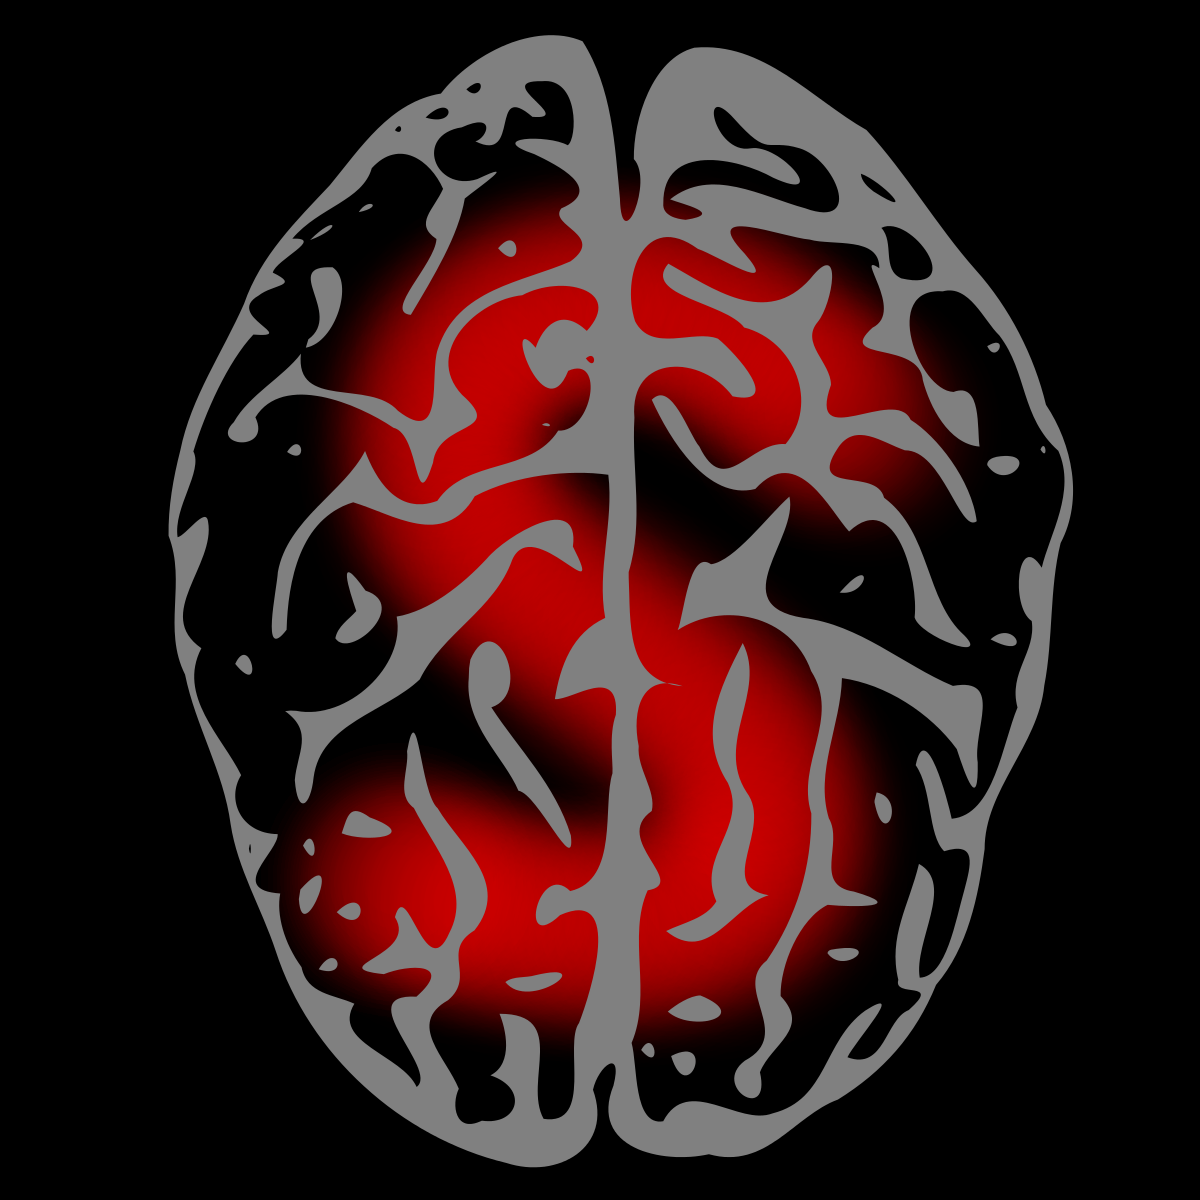
\includegraphics[scale = 0.035]{brain5.png} \\ \hline
\end{tabular}\\
\vspace{0.1in}
Test Data \\
\begin{tabular}{c|c|cccc}
\hline
 & & ? & ? & ? & ? \\
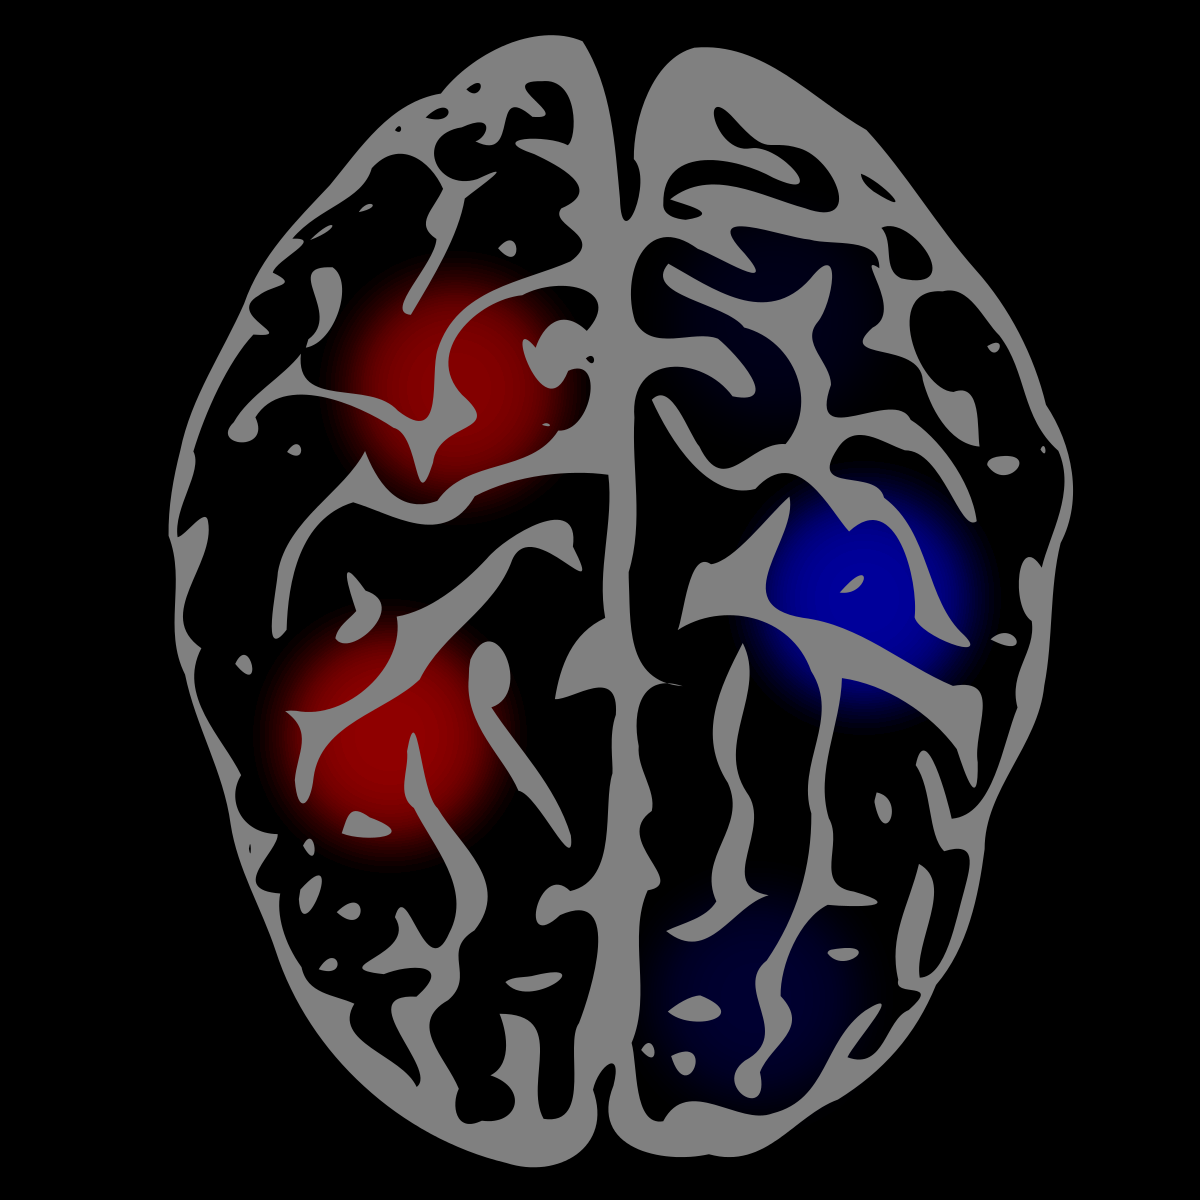
\includegraphics[scale = 0.035]{brain3.png} & \hspace{0.5in}
& 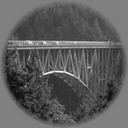
\includegraphics[scale = .26]{img1.png}
& 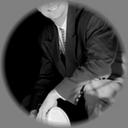
\includegraphics[scale = .26]{img2.png}
& 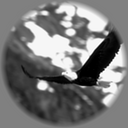
\includegraphics[scale = .26]{img3.png}
& 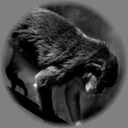
\includegraphics[scale = .26]{img4.png}\\
\hline
 & & ? & ? & ? & ? \\
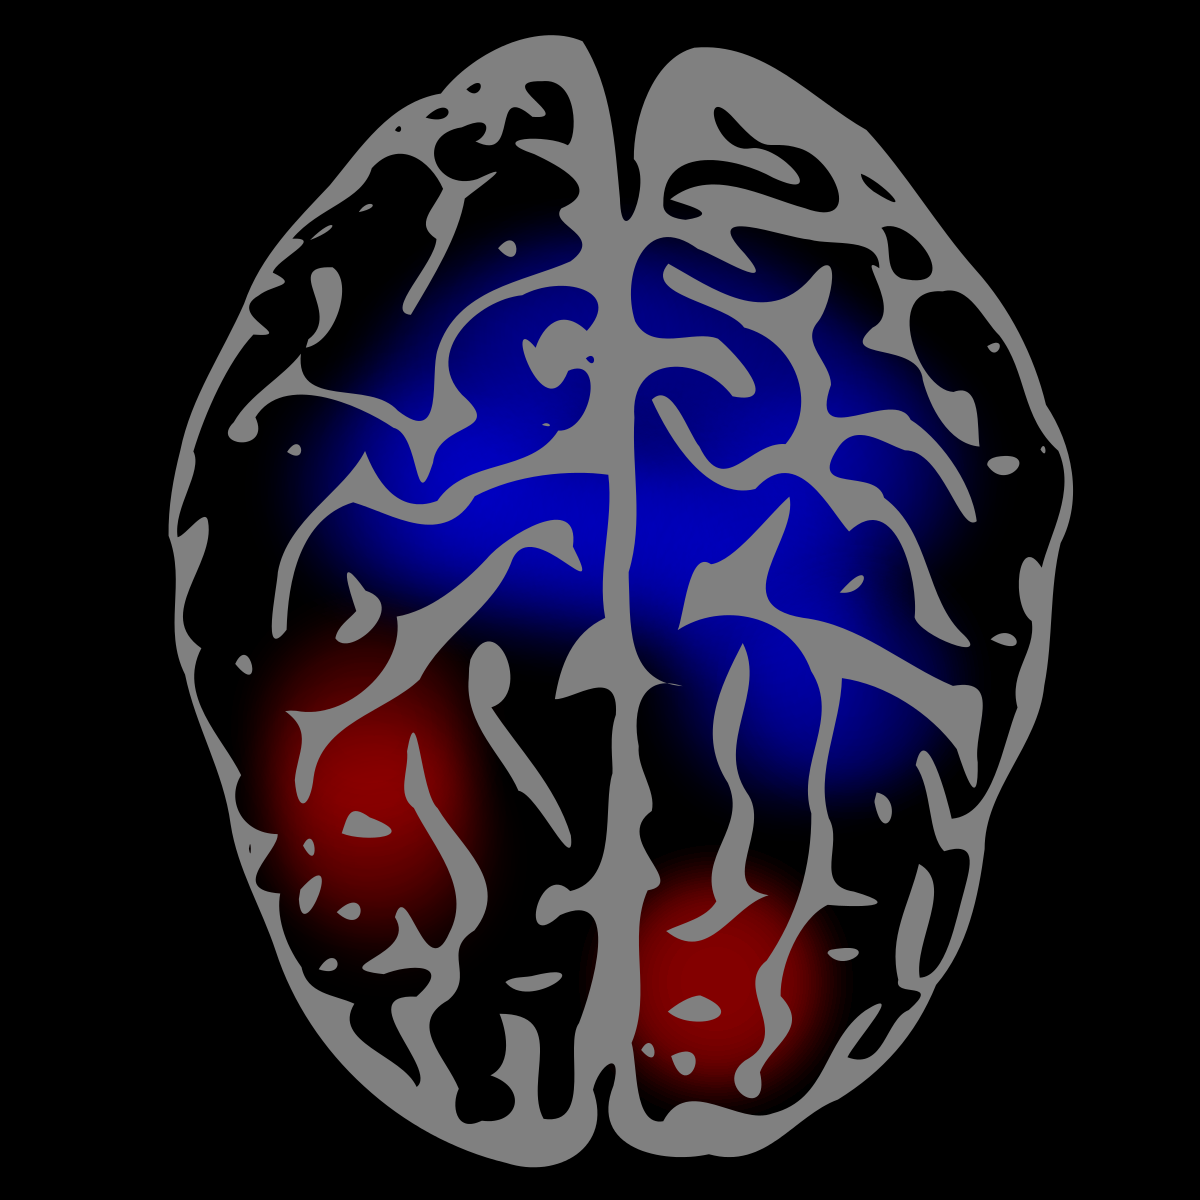
\includegraphics[scale = 0.035]{brain1.png} & \hspace{0.5in}
& 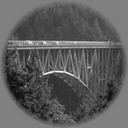
\includegraphics[scale = .26]{img1.png}
& 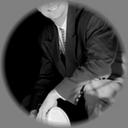
\includegraphics[scale = .26]{img2.png}
& 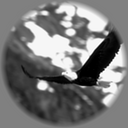
\includegraphics[scale = .26]{img3.png}
& 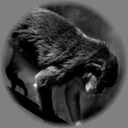
\includegraphics[scale = .26]{img4.png}\\
\hline
\end{tabular}
\end{center}
\end{frame}

\begin{frame}
\frametitle{Kay et al}
\begin{center}
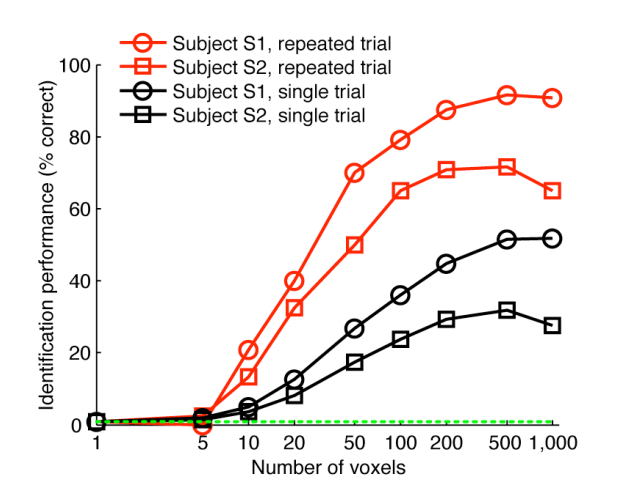
\includegraphics[scale=0.3]{kay_s4.png}
\end{center}
Redundancy of neural coding
\end{frame}

\begin{frame}
\frametitle{Kay et al}
\begin{center}
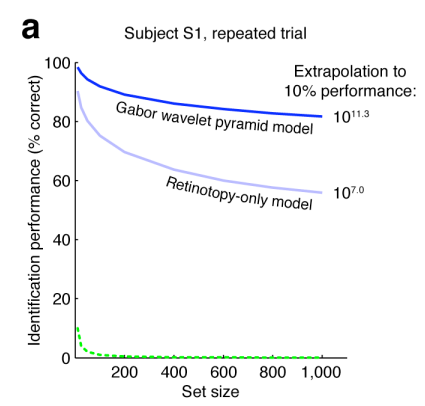
\includegraphics[scale=0.4]{kay_s5.png}
\end{center}
Can we extrapolate the classification curve?
\end{frame}

\section{Information theory}
{
\setbeamercolor{background canvas}{bg=}
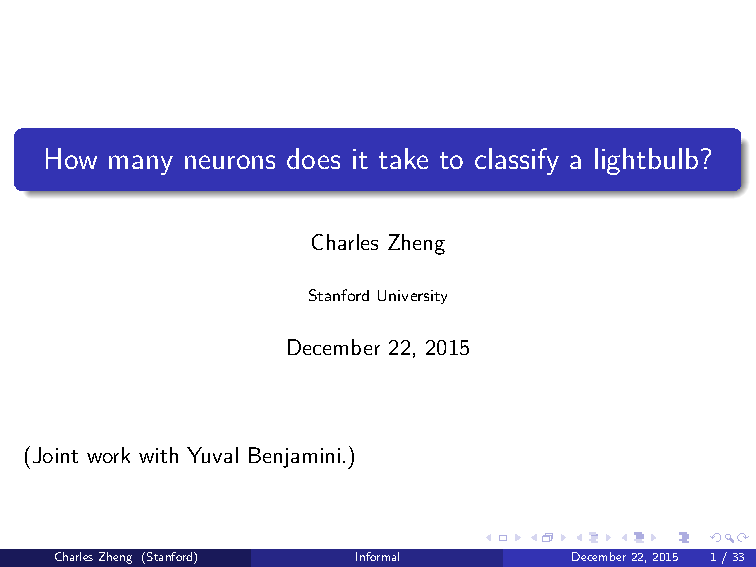
\includepdf[pages=1]{Zheng_mi_Jan.pdf}
}

\begin{frame}
\frametitle{Experimental design}
Sample stimuli iid from $p(\bx)$. Repeated measures.
\begin{center}
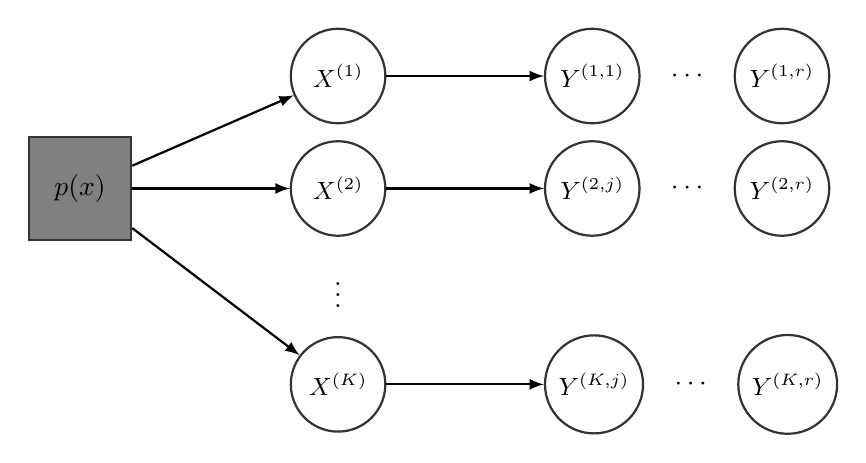
\begin{tikzpicture}[node distance = 2mm and 20mm]
\tikzstyle{main} = [circle, minimum size = 12mm, thick, draw = black!80]
\tikzstyle{main0} = [circle, minimum size = 2mm, thick, draw = white!100]
\tikzstyle{param} = [rectangle, minimum size = 13mm, thick, draw = black!80]
\tikzstyle{connect} = [-latex, thick]
\tikzstyle{box} = [rectangle, draw = black!100]
  \node[param, fill = black!50] (px) {$p(\bx)$};
  \node[main, right=of px] (x2) {\small{$\bX^{(2)}$}};
  \node[main, above=of x2] (x1) {\small{$\bX^{(1)}$}};
  \node[main0, below=of x2] (xdots) {$\vdots$};
  \node[main, below=of xdots] (x3) {\small{$\bX^{(K)}$}};
  \node[main, right=of x1] (y11) {\small{$\bY^{(1,1)}$}};
  \node[main, right=of x2] (y21) {\small{$\bY^{(2,j)}$}};
  \node[main, right=of x3] (y31) {\small{$\bY^{(K,j)}$}};
\begin{scope}[node distance = 3mm and 2mm]
  \node[main0, right=of y11] (y12) {$\cdots$};
  \node[main0, right=of y21] (y22) {$\cdots$};
  \node[main0, right=of y31] (y32) {$\cdots$};
  \node[main, right=of y12] (y13) {\small{$\bY^{(1,r)}$}};
  \node[main, right=of y22] (y23) {\small{$\bY^{(2,r)}$}};
  \node[main, right=of y32] (y33) {\small{$\bY^{(K,r)}$}};
\end{scope}
\path (px) edge [connect] (x1) (px) edge [connect] (x2) (px) edge [connect] (x3)
      (x1) edge [connect] (y11) (x2) edge [connect] (y21) (x3) edge [connect] (y31);
\end{tikzpicture}
\end{center}
\begin{itemize}
\item Main question: How to estimate $I(\bX;\bY)$ from such data?
\item Side question (experimental design): How to choose $K$?
\end{itemize}
\end{frame}

\begin{frame}
\frametitle{Entropy and mutual information}
$X$ and $Y$ have joint density $p(x, y)$ with respect to $\mu$.

\vspace{0.5in}

\begin{tabular}{c|c|c}
\hline
Quantity & Definition & Linear analogue\\\hline
Entropy & $H(X) = - \int (\log p(x)) p(x) \mu_X(dx)$ & $\text{Var}(X)$\\
Conditional entropy & $H(X|Y) = \E[H(X|Y)]$ & $\E[\text{Var}(X|Y)]$\\
Mutual information & $I(X;Y) = H(X) - H(X|Y)$ & $\text{Cor}^2(X, Y)$\\\hline
\end{tabular}

\vspace{0.3in}

\small{The above definition includes both \emph{differential} entropy and \emph{discrete} entropy.
Information theorists tend to use log base 2, we will use natural logs in this talk.}
\end{frame}

\begin{frame}
\frametitle{Can we learn $I(\bX; \bY)$ from such data?}
Answer: yes.
\begin{itemize}
\item We have $I(\bX; \bY) = H(\bY) - H(\bY|\bX)$.
\item We can estimate $H(\bY)$ from the data
\item We can estimate $H(\bY| \bx^{(i)})$ from the data, and define
\[
\hat{H}(\bY|\bX) = \frac{1}{K}\sum_{i=1}^K \hat{H}(\bY| \bX^{(i)})
\]
\item As $K$ and $r$ both tend to infinity,
\[
\hat{I}(\bX; \bY) = \hat{H}(\bY) - \hat{H}(\bY|\bX)
\]
is consistent for $I(\bX; \bY)$.
\end{itemize}
\end{frame}

\begin{frame}
\frametitle{Limitations with the `na\"{i}ve' approach}
Na\"{i}ve estimator:
\[
\hat{I}(\bX; \bY) = \hat{H}(\bY) - \frac{1}{K}\sum_{i=1}^K \hat{H}(\bY| \bX^{(i)})
\]
\begin{itemize}
\item If $K$ is small, the na\"{i}ve estimator may be quite biased, even for low-dimensional problems.
Gastpar et al. (2010) introduced an \emph{antropic correction} to deal with the small-$K$ bias.
\item Difficult to estimate differential entropies $H(\bY),\
  H(\bY|\bx^{(i)})$ in high dimensions.  Best rates are
  $O(1/\sqrt{n})$ for $d \leq 3$ dimensions.  Convergence rates for $d > 3$
  unknown!
\end{itemize}
\end{frame}

\begin{frame}
\frametitle{Can we use machine learning to deal with dimensionality?}
\begin{itemize}
\item Supervised learning becomes an extremely common approach for dealing with high-dimensional data, for numerous reasons!
\item Perhaps we can use supervised learning to estimate $I(\bX; \bY)$ as well.
\item Existing approach uses confusion matrix (Treves et al, 1997)
\end{itemize}
\end{frame}

\begin{frame}
\frametitle{Why use supervised learning to estimate $I(\bX; \bY)$?}

\begin{itemize}
\item Successful supervised learning exploits structure in the data, which \emph{nonparametric methods ignore.}
\item Using supervised learning to estimate mutual information can be viewed as \emph{using prior information} to improve the estimate of $I(\bX; \bY)$.
\item So while the general problem of information estimation is nearly impossible in high dimensions,
the problem might become tractable if we can exploit known structure in the problem!
\end{itemize}
\end{frame}

\begin{frame}
\frametitle{Relationship between mutual information and classification}
\begin{itemize}
\item Suppose $X$ and $Y$ are discrete random variables, and $X$ is uniformly distributed over its support.
\item Classify $X$ given $Y$.  The optimal rule is to guess
\[
\hat{X} = \argmax_x\ p(Y|X=x).
\]
\item Bayes error:
\[
p_e = \Pr[X \neq \hat{X}].
\]
\item Fano's inequality:
\[
I(X; Y) \geq (1-p_e) \ln K - \text{const.}
\]
where $K$ is the size of the support of $X$.
\end{itemize}
\end{frame}

\begin{frame}
\frametitle{Key Result}
Define the $K$-class \emph{average Bayes error} as
\[
ABE_K = \E[\Pr[\hat{X}_{Bayes}(Y) \neq X]]
\]
where $\hat{X}_{Bayes}$ is the optimal classification rule,
and the expectation averages over randomness in
$\bX^{(1)},\hdots, \bX^{(k)}$.

\vspace{0.3in}

Then, under a certain asymptotic regime,
there is an \emph{exact} relationship between $ABE_K$ and $I(\bX;\bY)$
(in contrast to the lower bound given by Fano's inequality or confusion matrix method.)

\end{frame}







\begin{frame}
\frametitle{Low SNR theorem}

\textbf{Theorem. }\emph{
Take a sequence of joint distributions $(\bX, \bY)$ where
the dimensionality of $\bX$ and $\bY$ grow to infinity,
but where
\[\lim I(\bX; \bY) = \iota < \infty.\]
Under certain regularity conditions, the limiting $K$-class average Bayes error is given by
\[
\lim_{d \to \infty} \text{ABE}_K = \pi_K(\sqrt{2\iota}).
\]
where
\[
\pi_K(\mu) =  1 - \int_{-\infty}^\infty \phi(z-\mu) (1-\Phi(z))^{K-1} dz.
\]
}
\end{frame}

{
\setbeamercolor{background canvas}{bg=}
\includepdf[pages=25]{Zheng_mi_Jan.pdf}
}


\begin{frame}
\frametitle{Regularity Conditions}
\begin{itemize}
\item We require the conditional log-likelihoods
\[
\log p(\bY^{(i)}|\bX^{(j)})
\]
to have a nondegenerate jointly multivariate normal limiting distribution (when scaled appropriately).
\item Define
\[
u(x, y) = \frac{p(x, y)}{p(x)p(y)} - 1.
\]
Draw $\bX \sim p(x)$ and $\bY^* \sim p(y)$ independently.
We require $u(\bX, \bY^*)$ have a
nondegenerate univariate normal limiting distribution (when scaled appropriately).  Also, $\Cov[u(\bX^{(i)}, \bY^{(j)}), u(\bX^{(k)}, \bY^{(j)})] \to 0.$
\end{itemize}
These conditions are satisfied quite generally, e.g. if $(\bX, \bY)$ multivariate normal with limiting spectrum.
\end{frame}

\begin{frame}
\frametitle{The low-SNR estimator of $I(\bX;\bY)$}

Our proposed estimator for mutual information is
\[
\hat{I}_{ls}(\bX; \bY) = \frac{1}{2}\pi_K^{-1}(\widehat{\text{ABE}})^2
\]
where $\widehat{\text{ABE}}$ is the test error of the classifier.
(The subscript $ls$ stands for low-SNR.)

\vspace{0.3in}

Note: there is still a lot of improvement for this estimator,
mainly correcting for bias due to variability in $\widehat{\text{ABE}}$.
This is the first version we tried.

\end{frame}

{
\setbeamercolor{background canvas}{bg=}
\includepdf[pages=32-34]{Zheng_mi_Jan.pdf}
\includepdf[pages=37]{Zheng_mi_Jan.pdf}
\includepdf[pages=39]{Zheng_mi_Jan.pdf}}
\section{RSA}
{
\setbeamercolor{background canvas}{bg=}
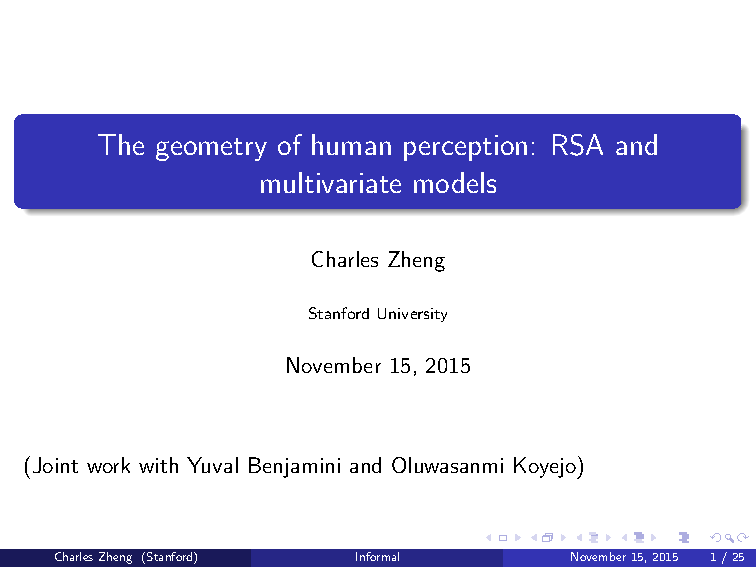
\includepdf[pages=1]{Zheng_rsa_Nov17.pdf}
\includepdf[pages=3-7]{Zheng_rsa_Nov17.pdf}
\includepdf[pages=15]{Zheng_rsa_Nov17.pdf}
\includepdf[pages=19-20]{Zheng_rsa_Nov17.pdf}
\includepdf[pages=4]{Zheng_Oct29.pdf}
}

\begin{frame}
\frametitle{Parametric RSA}
\begin{itemize}
\item Combine the parametric approach of multivariate regression with RSA.
\item Model:
\[
y \sim N(B^T x, \Omega^{-1}).
\]
\item The distribution-induced metric is therefore
\[
D(x_i, x_j) = (x_i - x_j)^T B \Omega B^T (x_i - x_j).
\]
\end{itemize}
\end{frame}

\begin{frame}
\frametitle{Parametric RSA}
\[
y \sim N(B^T x, \Omega^{-1})
\]
\[
D(x_i, x_j) = (x_i - x_j)^T B \Omega B^T (x_i - x_j)
\]
\begin{itemize}
\item Since all information about the distance is captured by the matrix $\Sigma = B\Omega B^T$, instead of testing
\[
D^A = D^B
\]
we can test
\[
\Sigma^A = \Sigma^B.
\]
\item We can compare two datasets with non-overlapping stimuli
\item The approach is scalable in the number of distinct stimuli,
  since the size of $\Sigma^A$, $\Sigma^B$ only depend on the number of
  \emph{features} rather than the number of stimuli
\end{itemize}
\end{frame}

{
\setbeamercolor{background canvas}{bg=}
\includepdf[pages=7-8]{sketch.pdf}
}

\begin{frame}
\frametitle{Comparison with information approach}
\begin{itemize}
\item Parametric RSA makes strong assumptions on the model (e.g. linearity.)
\item We can track information loss: $I(X; Y^{V1}) > I(X; Y^{V2})$
\item But in cases of \emph{selective transmission},
we can infer \emph{which dimensions of information} are being lost
(face features, house features, etc.)
\item We get a finer-grained picture of information flow than the Shannon information approach.
\end{itemize}
\end{frame}

\section{To do}

\frame{\sectionpage}

\begin{frame}
\frametitle{Ongoing}
\begin{itemize}
\item Apply low-SNR information estimator and parametric RSA to real data.
\item Develop bootstrap-based hypothesis tests for parametric RSA: e.g. $H_0: \Sigma^A = \Sigma^B$.
\end{itemize}
\end{frame}

\begin{frame}
\frametitle{Possible extensions of information theory work}
\begin{itemize}
\item Our proposed estimator performs well in small sample sizes, yet is \emph{not consistent}... can it be fixed?
\item Develop complimentary theory for estimating Bayes error.
(This would allow us to state risk bounds for estimating $I(X; Y)$.)
\item Even if you don't care about Shannon information, the theory allows you to potentially
extrapolate classification curves:
\[
ABE_{10} \to I(X; Y) \to ABE_{10000}
\]
(But more work is needed.)
\item Use our theory to address the question of optimal experimental design.
\end{itemize}
\end{frame}

\begin{frame}
\frametitle{Possible extensions of RSA work}
Beyond testing $\Sigma^A = \Sigma^B$
\begin{itemize}
\item Inference on which components of $\Sigma^A$ differ from $\Sigma^B$.
\item Multiple comparisons: comparing $\Sigma^A$ to $\Sigma^B$ to $\Sigma^C$
\item Inferring latent features $X$ from data!  \emph{Multiple MDS}
\[
\min_{x, \Sigma^k} \sum_{i,j,k} w_{ijk} (D^k_{ij} - (x_i - x_j)^T \Sigma^k (x_i - x_j)).
\]
\end{itemize}
\end{frame}

{
\setbeamercolor{background canvas}{bg=}
\includepdf[pages=8]{sketch.pdf}
}

\begin{frame}
\frametitle{References}
\begin{itemize}
\item Kay, KN., Naselaris, T., Prenger, R. J., and Gallant, J. L.
  ``Identifying natural images from human brain
  activity''. \emph{Nature} (2008)
\item Naselaris, et al. ``Bayesian reconstruction of natural images
  from human brain activity''.  \emph{Neuron} (2009)
\item Vu, V. Q., Ravikumar, P., Naselaris, T., Kay, K. N., and Yu, B.
  ``Encoding and decoding V1 fMRI responses to natural images with
  sparse nonparametric models'', \emph{The Annals of Applied
    Statistics}. (2011)
\item Chen, M., Han, J,. Hu, X., Jiang, Xi., Guo, L. and Liu, T.
  ``Survey of encoding and decoding of visual stimulus via fMRI: an
  image analysis perspective.'' \emph{Brain Imaging and
    Behavior}. (2014)
\end{itemize}
\end{frame}

\begin{frame}
\frametitle{References}
\begin{itemize}
\item Cover and Thomas.  Elements of information theory.
\item Gastpar., Gill., Huth., Theunnisen.  ``Anthropic Correction of Information Estimates and Its Application to Neural Coding.'' IEEE Trans I.T.
\item Quiroga and Panzeri. ``Extracting information from neuronal populations: information theory and decoding approaches.''  Nature Rev. Neuro.
\item Muirhead.  Aspects of multivariate statistical theory.
\item van der Vaart.  Asymptotic statistics.
\end{itemize}
\end{frame}

\begin{frame}
\frametitle{References}
\begin{itemize}
\item Kriegeskorte, N. (2008). Representational similarity analysis – connecting the branches of systems neuroscience. Frontiers in Systems Neuroscience
\item Kriegeskorte, N., \& Bandettini, P. (2007). Analyzing for information, not activation, to exploit high-resolution fMRI. NeuroImage, 38(4), 649–662. doi:10.1016/j.neuroimage.2007.02.022
\item Kay, K. N., Naselaris, T., Prenger, R. J., \& Gallant, J. L. (2008). Identifying natural images from human brain activity. Nature, 452(March), 352–355. doi:10.1038/nature06713
\item Guillot, G., \& Rousset, F. (2013). Dismantling the Mantel tests. Methods in Ecology and Evolution, 4(4), 336–344. doi:10.1111/2041-210x.12018
\item Cole, M. W., Reynolds, J. R., Power, J. D., Repovs, G., Anticevic, A., \& Braver, T. S. (2013). Multi-task connectivity reveals flexible hubs for adaptive task control. Nature Neuroscience, 16(9), 1348–1355. doi:10.1038/nn.3470
\end{itemize}
\end{frame}


\end{document}
